\documentclass[journal,12pt,twocolumn]{IEEEtran}
%

\usepackage{setspace}
\usepackage{gensymb}
\singlespacing

\usepackage{amsmath}
\usepackage{amsthm}
\usepackage{txfonts}
\usepackage{cite}
\usepackage{enumitem}
\usepackage{mathtools}
\usepackage{listings}
    \usepackage{color}                                            %%
    \usepackage{array}                                            %%
    \usepackage{longtable}                                        %%
    \usepackage{calc}                                             %%
    \usepackage{multirow}                                         %%
    \usepackage{hhline}                                           %%
    \usepackage{ifthen}                                           %%
  %optionally (for landscape tables embedded in another document): %%
    \usepackage{lscape}     
\usepackage{multicol}
\usepackage{chngcntr}
\usepackage{float}
\renewcommand\thesection{\arabic{section}}
\renewcommand\thesubsection{\thesection.\arabic{subsection}}
\renewcommand\thesubsubsection{\thesubsection.\arabic{subsubsection}}

\renewcommand\thesectiondis{\arabic{section}}
\renewcommand\thesubsectiondis{\thesectiondis.\arabic{subsection}}
\renewcommand\thesubsubsectiondis{\thesubsectiondis.\arabic{subsubsection}}

% correct bad hyphenation here
\hyphenation{op-tical net-works semi-conduc-tor}
\def\inputGnumericTable{}                                 %%

\lstset{
%language=C,
frame=single, 
breaklines=true,
columns=fullflexible
}

\begin{document}
%


\newtheorem{theorem}{Theorem}[section]
\newtheorem{problem}{Problem}
\newtheorem{proposition}{Proposition}[section]
\newtheorem{lemma}{Lemma}[section]
\newtheorem{corollary}[theorem]{Corollary}
\newtheorem{example}{Example}[section]
\newtheorem{definition}[problem]{Definition}
\newcommand{\BEQA}{\begin{eqnarray}}
\newcommand{\EEQA}{\end{eqnarray}}
\newcommand{\define}{\stackrel{\triangle}{=}}
\bibliographystyle{IEEEtran}
\providecommand{\mbf}{\mathbf}
\providecommand{\pr}[1]{\ensuremath{\Pr\left(#1\right)}}
\providecommand{\qfunc}[1]{\ensuremath{Q\left(#1\right)}}
\providecommand{\sbrak}[1]{\ensuremath{{}\left[#1\right]}}
\providecommand{\lsbrak}[1]{\ensuremath{{}\left[#1\right.}}
\providecommand{\rsbrak}[1]{\ensuremath{{}\left.#1\right]}}
\providecommand{\brak}[1]{\ensuremath{\left(#1\right)}}
\providecommand{\lbrak}[1]{\ensuremath{\left(#1\right.}}
\providecommand{\rbrak}[1]{\ensuremath{\left.#1\right)}}
\providecommand{\cbrak}[1]{\ensuremath{\left\{#1\right\}}}
\providecommand{\lcbrak}[1]{\ensuremath{\left\{#1\right.}}
\providecommand{\rcbrak}[1]{\ensuremath{\left.#1\right\}}}
\theoremstyle{remark}
\newtheorem{rem}{Remark}
\newcommand{\sgn}{\mathop{\mathrm{sgn}}}
\providecommand{\abs}[1]{\left\vert#1\right\vert}
\providecommand{\res}[1]{\Res\displaylimits_{#1}} 
\providecommand{\norm}[1]{\left\lVert#1\right\rVert}
\providecommand{\mtx}[1]{\mathbf{#1}}
\providecommand{\mean}[1]{E\left[ #1 \right]}
\providecommand{\fourier}{\overset{\mathcal{F}}{ \rightleftharpoons}}
\providecommand{\system}{\overset{\mathcal{H}}{ \longleftrightarrow}}


\newcommand{\myvec}[1]{\ensuremath{\begin{pmatrix}#1\end{pmatrix}}}
\newcommand{\cmyvec}[1]{\ensuremath{\begin{pmatrix*}[c]#1\end{pmatrix*}}}
\newcommand{\mydet}[1]{\ensuremath{\begin{vmatrix}#1\end{vmatrix}}}
\newcommand{\proj}[2]{\textbf{proj}_{\vec{#1}}\vec{#2}}
\let\StandardTheFigure\thefigure
\let\vec\mathbf
 
\title{ASSIGNMENT 11}
\author{Gayathri S}
	

\maketitle
\renewcommand{\thefigure}{\theenumi}
\renewcommand{\thetable}{\theenumi}
  
   Download all python codes from 
\begin{lstlisting}
https://github.com/Gayathri1729/SRFP/tree/main/Assignment11
\end{lstlisting}
%
and latex-tikz codes from 
%
\begin{lstlisting}
https://github.com/Gayathri1729/SRFP/tree/main/Assignment11
\end{lstlisting}
%
\section{OPTIMIZATION 2.17}
A cottage industry manufactures pedestal
lamps and wooden shades, each requiring
the use of a grinding/cutting machine and a
sprayer. It takes 2 hours on grinding/cutting
machine and 3 hours on the sprayer to
manufacture a pedestal lamp. It takes 1 hour
on the grinding/cutting machine and 2 hours
on the sprayer to manufacture a shade. On any
day, the sprayer is available for at the most 20
hours and the grinding/cutting machine for at
the most 12 hours. The profit from the sale of
a lamp is Rs 5 and that from a shade is Rs
3. Assuming that the manufacturer can sell all
the lamps and shades that he produces, how
should he schedule his daily production in
order to maximise his profit?

\section{SOLUTION}

\begin{itemize}
\item All the data can be tabularised as:
\numberwithin{table}{section}
\begin{table}[!ht]
\centering
\resizebox{\columnwidth}{!}{\begin{tabular}{|c|c|c|c|} 
\hline
 & Grinding machine&Sprayer&Profit\\
\hline
\textbf{Pedestal lamps} & 2 & 3 & 5 \\ 
\hline
\textbf{Wooden shades} & 1  & 2 & 3 \\ 
\hline
\text{Max Hours} & $\leq12$&$\leq20$&\\
\hline
\end{tabular}}
\caption{Time needed and Profit for each object}
\label{tab:table1}
\end{table}
\item Let the number of pieces of pedestal lamp manufactured be $x$ and
the number of pieces of wooden shades manufactured be $y$ such that : 
\begin{align}
    x \geq 0 
    \\
    y \geq 0 
\end{align}
\item From the data given we have:
\begin{align}
    2x+y &\leq 12 
\end{align}
and,
\begin{align}
    3x+2y &\leq  20
\end{align}
$\therefore$ The maximizing function is:
\begin{align}
        \max Z &= \myvec{5& 3}\vec{x}\\
        s.t. \quad 
        \myvec{2 & 1\\ 3 & 2 }\vec{x} &\preceq \myvec{12\\20} \\
        \vec{-x} &\preceq \vec{0}
\end{align}
\item The Lagrangian function can be given as:
\begin{equation}
\begin{aligned}
    &L(\vec{x},\boldsymbol{\lambda}) \\ &= \myvec{5 & 3}\vec{x}+\lcbrak{\sbrak{\myvec{2 & 1}\vec{x}-12}} \\ &+ \sbrak{\myvec{3 & 2}\vec{x}-20} \\ &+ \sbrak{\myvec{-1 & 0}\vec{x}} +\rcbrak{\sbrak{\myvec{0 & -1}\vec{x}}}\boldsymbol{\lambda}
\end{aligned}
\end{equation}
where,
\begin{align}
    \boldsymbol{\lambda} &= \myvec{\lambda_1 \\ \lambda_2 \\ \lambda_3 \\ \lambda_4}
\end{align}
\item Now, we have
\begin{align}
    \nabla L(\vec{x},\boldsymbol{\lambda}) &= \myvec{5 + \myvec{2 & 3 & -1 & 0 }\boldsymbol{\lambda}\\ 3 +\myvec{1 & 2 &0 & -1}\boldsymbol{\lambda} \\ \myvec{2 & 1}\vec{x}-12 \\ \myvec{3 & 2}\vec{x}-20 \\ \myvec{-1 & 0}\vec{x} \\ \myvec{0 & -1}\vec{x}}
\end{align}
$\therefore$ The Lagrangian matrix is given by:-
\begin{align}
  \small{\myvec{0 & 0 & 2 & 3 & -1 & 0 \\ 0 & 0 & 1 & 2 &0 & -1 \\ 2 & 1 & 0 & 0 & 0 & 0 \\ 3 & 2 & 0 & 0 & 0 & 0 \\ -1 & 0 & 0 & 0 & 0 & 0 \\ 0 & -1 & 0 & 0 & 0 & 0 }\myvec{\vec{x} \\ \boldsymbol{\lambda} }}= \small{\myvec{-5 \\ -3 \\ 12 \\ 20 \\ 0 \\0 }}
\end{align}
\item Considering $\lambda_1,\lambda_2$ as only active multiplier,
\begin{align}
    \myvec{0 & 0 & 2 & 3  \\ 0 & 0 & 1 & 2 \\ 2 & 1 & 0 & 0 \\3 & 2 & 0 & 0}\myvec{\vec{x}\\ \boldsymbol{\lambda}} &= \myvec{-5 \\ -3 \\ 12 \\ 20}
\end{align}
\begin{align}
 \implies   \myvec{\vec{x} \\ \boldsymbol{\lambda}} &=  \myvec{0 & 0 & 2 & 3  \\ 0 & 0 & 1 & 2 \\ 2 & 1 & 0 & 0 \\3 & 2 & 0 & 0} ^{-1}\myvec{-5 \\ -3 \\ 12 \\ 20}
    \\
    \implies   \myvec{\vec{x} \\ \boldsymbol{\lambda}} &= \myvec{0 & 0 & 2 & -1 \\ 0 & 0 & -3 & 2 \\ 2 & -3 & 0 & 0 \\ -1 & 2 & 0 & 0}\myvec{-5 \\ -3 \\ 12 \\ 20}
    \\
    \implies \myvec{\vec{x} \\ \boldsymbol{\lambda}} &= \myvec{4\\24 \\ -1 \\ -1 }
\end{align}
$\because \boldsymbol{\lambda}=\myvec{-1 \\ -1} \prec \vec{0}$
\\
\item The Optimal solution is given by:
\begin{align}
    \vec{x} &= \myvec{4\\4} \\
    Z &= \myvec{5&3}\vec{x} \\
   Z &= \myvec{5&3}\myvec{4 \\ 4} \\
    Z&= \text{Rs.} 32
\end{align}
\item So, to maximise profit
\\
 No. of pedestal lamps manufactured is \boxed{x=4} and
 
 No. of wooden shades manufactured is \boxed{y=4}.
\item The maximum daily profit is \boxed{Z=\text{Rs.} 32} .
\numberwithin{figure}{section}
\begin{figure}[!ht]
\centering
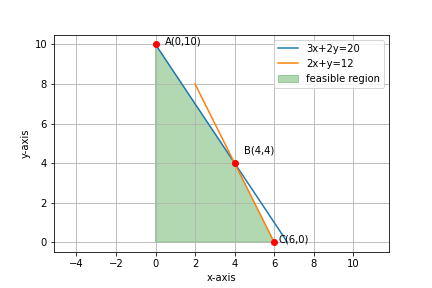
\includegraphics[width=\columnwidth]{assignment11.png}
\caption{Graphical Representataion}
\end{figure}
\end{itemize}
\end{document}
